\\[0.1in]
\begin{enumerate}
    \item[1.]
    \begin{enumerate}
        \item[(آ)]
        رابطه $R$، یک رابطه هم‌ارزی\LTRfootnote{equivalence relation}
        می‌باشد. می‌دانیم رابطه $R$ زمانی یک رابطه هم‌ارزی است که شروط زیر را داشته باشد:
        \begin{latin}
        \begin{center}
            \begin{itemize}
                \item R is reflexive:\\
                    \begin{center}
                        $\forall \; x \in A, \;\;\; xRx.$
                    \end{center}
                \item R is symmetric:\\
                    \begin{center}
                        $\forall \; x,y \in A, \;\;\; 
                        xRy \; \rightarrow \; yRx.$
                    \end{center}
                \item R is transitive:\\
                    \begin{center}
                        $\forall \; x, y, z \in A,\;\;\; 
                        xRy \; \textit{and} \; yRz
                        \; \rightarrow xRz.$\\[0.15in]
                    \end{center}
            \end{itemize}
        \end{center}
        \end{latin}
        \newpage
        حال قبل از اینکه به رابطه $R$ بپردازیم، یک موضوع بدیهی را شرح می‌دهیم.
        می‌دانیم رابطه تساوی
        \LTRfootnote{is equal to or =}
        ، یک رابطه هم‌ارزی می‌باشد.\\
        \begin{latin}
            \centering
                \begin{enumerate}
                    \item[1.]
                    \text{(Reflexivity)} \; $x = x,$
                    \item[2.]
                    \text{(Symmetry)} \;\; $x\;=\;y \;\;
                    \rightarrow \; y\;=\;x,$
                    \item[3.]
                    \text{(Transitivity)} \;
                    $x\;=\;y \; \textit{and} \; y\;=\;z
                        \; \rightarrow \; x\;=\;z.$
                \end{enumerate}
        \end{latin} 
        اکنون به سراغ رابطه $R$ می‌رویم:\\[0.2in]
        \begin{itemize}
            \item 
            ویژگی اول:
        \begin{center}
            $\forall \; a, b \in A,$\\
            $(a, b)R(a,b) \Leftrightarrow \sin a \cos b = \sin a \cos b$\\[0.15in]
        \end{center}
        طبق اینکه رابطه تساوی، ویژگی $reflexivity$ را داراست،
        بنابراین
        $(a,b)R(a,b)$
        درست می‌باشد و $R$ ویژگی $reflexivity$ را دارا است.\\[0.15in]
            \item 
            ویژگی دوم:\\[0.15in]
            می‌دانیم اگر $(a,b)R(c,d)$،
            یعنی $\sin a \cos b = \sin c \cos d$.
            پس طبق ویژگی $symmetry$ برای رابطه تساوی، نتیجه می‌گیریم که 
            $\sin c \cos d = \sin a \cos b$.
            که همان $(c,d)R(a,b)$ می‌باشد.
            در نتیجه داریم:\\[0.05in]
            \begin{center}
                $(a,b)R(c,d) \rightarrow (c,d)R(a,b)$\\[0.2in]
            \end{center}
            \item 
            ویژگی سوم:\\[0.15in]
            در نظر بگیرید:\\[0.05in]
            \begin{center}
                $\forall \;a,b,c,d,e,f \in A,\;\;\;
                (a,b)R(c,d)\;\; \textit{and} \;\; (c,d)R(e,f)$\\[0.1in]
                $\Longrightarrow 
                \sin a \cos b = \sin c \cos d$\\[0.1in]
                $\Longrightarrow 
                \sin c \cos d = \sin e \cos f$\\[0.1in]
                $\xrightarrow{transitivity\; of\; "="}\;
                \sin a \cos b = \sin e \cos f
                \rightarrow
                (a,b)R(e,f)$\\[0.15in]
            \end{center}
            به روش دیگری نیز می‌توانیم این ویژگی را اثبات نماییم:
            \begin{center}
                \begin{equation}
                    \label{one}
                    \sin a \cos b = \sin c \cos d
                \end{equation}
                \begin{equation}
                    \label{two}
                    \sin c \cos d = \sin e \cos f
                \end{equation}
                \\[0.15in]
            \end{center}
            حال با ضرب کردن \ref{one} در \ref{two} داریم:\\[0.1in]
            \begin{center}
                $\sin a \cos b \; \sin c \cos d = 
                \sin c \cos d \; \sin e \cos f$\\[0.15in]
            \end{center}
            اگر مقدار
            $\sin c \cos d$ صفر باشد، که تمامی عبارت‌ها صفر هستند و برابری ثابت می‌شود. در غیر این‌صورت با تقسیم دو طرف معادله بر
            $\sin c \cos d$
            داریم:\\[0.1in]
            \begin{center}
                $\sin a \cos b = 
                \sin e \cos f$\\[0.15in]
            \end{center}
            بنابراین رابطه $R$ ویژگی سوم را نیز دارا می‌باشد.\\[0.2in]
        \end{itemize}
        در نتیجه این رابطه، یک رابطه هم‌ارزی است.\\[0.15in]
        \item[(ب)]
        رده هم‌ارزی یا همان کلاس هم‌ارزی $a$ تحت رابطه $R$، برابر تمام $b$هایی است که:
        \\[0.1in]
        \begin{center}
            $aRb$
        \end{center}
        بنابراین در این سوال باید $a$ و $b$هایی را بیابیم که:\\[0.1in]
        \begin{center}
            $(30, 60)R(a, b) \Leftrightarrow
            \sin(30)\cos(60) = \sin a \cos b$\\[0.1in]
            $\longrightarrow \sin a \cos b = \frac{1}{4}$
        \end{center}
        با توجه به $A$ داریم:\\[0.1in]
        \[
    \sin(30)\cos(60) = \left\{\begin{array}{lr}
        \sin(330)&\cos(240)\\
            \sin(330)&\cos(120)\\
            \sin(210)&\cos(240)\\
            \sin(210)&\cos(120)\\
            \sin(150)&\cos(300)\\
            \sin(150)&\cos(60)\\
            \sin(30)&\cos(300)\\
            \sin(30)&\cos(60)\\
        \end{array}\right\} = \frac{1}{4}\\[0.15in]
  \]
    بنابراین رده هم‌ارزی 
    $[(30, 60)]$ برابر است با:
\begin{center}
    $\{(30,60), (30, 300), (150, 60), (150, 300), (210,120)
    , (210, 240), (330, 120), (330, 240)\}$\\[0.2in]
\end{center}
    \end{enumerate}
    \item[2.]
    ابتدا دو تعریف را یادآوری می‌نماییم:\\[0.1in]
    \begin{latin}
        \begin{itemize}
            \item The inverse relationship of R is denoted by $R^{-1}$\\[0.05in]
            \begin{center}
                $R^{-1} = \{(y,x)\; |\; (x,y) \; \in A\}$
            \end{center}
            \item 
            R is anti-symmetric:\\[0.05in]
            \begin{center}
                $\forall \; x,y\;\in A, \;\;
                xRy\;\textit{and}\;yRx\;
                \rightarrow\;
                x=y.$\\[0.1in]
            \end{center}
        \end{itemize}
    \end{latin}
    حال به شروع اثبات می‌پردازیم:\\[0.06in]
    \begin{enumerate}
        \item[1.] طرف اول:\\[0.1in]
        فرض کنید $R$ پادتقارنی است. اگر 
        $R \cap R^{-1}$ تهی یا $\varnothing$ باشد، که زیرمجموعه $\Delta$ می‌باشد و اثبات می‌شود.
        ( زیرا $\varnothing$ زیرمجموعه تمامی $set$ها می‌باشد.)
        حال فرض کنید $R \cap R^{-1}$ تهی نمی‌باشد و داریم:\\[0.07in]
        \begin{center}
            $(a,b) \;\in\; R \cap R^{-1} \longrightarrow
            (a,b)\in R\; \textit{and}\; (a,b)\in R^{-1}$\\[0.15in]
        \end{center}
        به کمک تعریفی که از $R^{-1}$ داریم:\\[0.01in]
        \begin{center}
            $(a,b)\in R^{-1} \longrightarrow (b,a)\in R$\\[0.08in]
            $\Longrightarrow (a,b)\in R,\;\;(b,a) \in R\;
            \xrightarrow{\textit{\lr{R is anti-symmetric}}}\; a=b$
            \\[0.1in]
        \end{center}
        در نتیجه اعضایی که در $R \cap R^{-1}$ هستند، به فرم $(a, a)$
        می‌باشند و از آنجا که 
        $(a,a)\in \Delta$،
        نتیجه می‌شود:\\[0.1in]
        \begin{center}
            $R \cap R^{-1} \; \subseteq\; \Delta$\\[0.1in]
        \end{center}
    \item[2.] طرف دوم: \\[0.1in]
    فرض کنید 
    $R \cap R^{-1} \; \subseteq\; \Delta$.
    حال درنظر بگیرید
    $(a,b)\in R$ و
    $(b,a)\in R$.
    با توجه به تعریف $R^{-1}$
    داریم:\\[0.1in]
    \begin{center}
        $(a,b)\in R^{-1}$\\[0.05in]
        $(b,a)\in R^{-1}$\\[0.15in]
    \end{center}
    یک عضو در اشتراک دو مجموعه قرار دارد اگر عضو هر دو مجموعه باشد، بنابراین:\\[0.05in]
    \begin{center}
        $(a,b)\in R \cap R^{-1}$\\[0.05in]
        $(b,a)\in R \cap R^{-1}$\\[0.05in]
        $\xrightarrow{R \cap R^{-1}\; \in \; \Delta}\;
        (a,b)\in \Delta, \;\; (b,a)\in \Delta$\\[0.08in]
    \end{center}
    حال طبق تعریف $\Delta$ داریم:\\[0.05in]
    \begin{center}
        $\Delta = \{(a, a)\; | \; a \in A \}\; \rightarrow\;
        a=b$\\[0.1in]
    \end{center}
    در نتیجه نشان دادیم که \text{anti-symmetric} می‌باشد.
    \end{enumerate}
    بنابراین به خواسته سوال رسیدیم و نشان دادیم که $R$ پادتقارنی است اگر وتنها اگر
    $R \cap R^{-1} \subseteq \Delta$ باشد.
    راه دیگر برای این سوال را در تصویر زیر مشاهده می‌فرمایید:
    \begin{figure} [H]
    \centering
    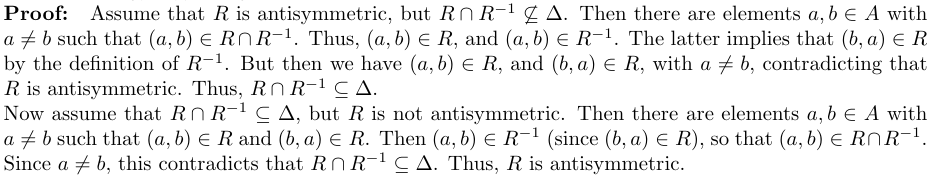
\includegraphics[scale=0.82]{solution/3.png}
\end{figure}
\end{enumerate}